\section{Performance} \label{sec:lhc:performance}

Since the begining of its stable running in 2010 the LHC has performed well,
exceeding expectations.  While the experiment itself is incredibly complex, the
performance of the machine, for the purposes of our analysis, can be reduced to
two numbers; the familiar center of mass energy of the beams and a less common
quantity known as the integrated luminosity.  

For particle physics the integrated luminosity is proportional to the total
number of collisions recorded during a specified time period, while the
instantaneous luminosity is proportional to the bunch crossing rate along with
the cross section of a proton-proton interaction and represents the potential
number of collisions per second.  Knowing this we can see that the integrated
luminosity, $L_{int}$ is simply the integral of the instantaneous luminosity
$L_{inst.}$ for a chosen data period as seen in
\Cref{eq:integrated_luminosity}.

\begin{equation} \label{eq:integrated_luminosity}
   L_{int} = \int L_{inst.}dt 
\end{equation}

For a standard Gaussian beam, $L_{inst.}$ can be written as

\begin{equation} \label{eq:inst_luminosity}
  L_{inst.} = \frac{N_{b}^{2}n_{b}f_{rev}\gamma_{r}}{4\pi\epsilon_{n}\beta^{*}}F
\end{equation}

where $N_{b}$ is the number of particles per bunch, $n_{b}$ the number of
bunches per beam, $f_{rev}$ the revolution frequency, $\gamma_{r}$ the
relativistic gamma factor, $\epsilon_{n}$ the normalized transverse beam
emittance, $\beta^{*}$ the beta function at the collision point, and $F$ the
geometric luminosity reduction factor due to the crossing angle at the
interaction point given by

\begin{equation}
  F = \bigg(1 + \Big( \frac{\theta_{c}\sigma_{z}}{2\sigma^{*}} \Big) ^{2}
\bigg)^{-1/2} 
\end{equation}

where $\theta_{c}$ is the full crossing angle at the interaction point,
$\sigma_{z}$ is the RMS bunch length, and $\sigma^{*}$ is the transverse RMS
beam size at the interaction point. Nominal values for the above quantities are
shown in \Cref{table:nominal_values} which also demonstrates the incredible
success of the LHC operators and accelerator teams during the LHC Run II data
taking period.

\begin{table}[htpb]
 \centering
 \caption{
  Nominal design values of LHC operations parameters at ATLAS for $25~\textrm{ns}$ bunch crossing spacing~\cite{Evans:2008zzb,PhysRevAccelBeams.19.101003}.
  Design and ATLAS recorded values of the machine luminosity are also given for LHC Run II operations~\cite{TWiki:2018ATLASPeakLumi}.
 }
 \begin{tabular}{@{}llr@{}} \toprule
  Parameter                                   & Symbol             & LHC Run II Value                \\ \midrule
  LHC circumference                           &                    & $26,659~\mathrm{m}$             \\
  LHC design beam energy                      &                    & $7~\TeV$                        \\
  LHC beam energy in Run II                   &                    & $6.5~\TeV$                      \\
  Number of protons per bunch                 & $N_{b}$            & $1.15 \times 10^{11}$           \\
  Number of proton bunches per beam           & $n_{b}$            & $2,808$                         \\
  Revolution frequency                        & $f_{\textrm{rev}}$ & $11.245~\mathrm{kHz}$           \\
  Lorentz factor (design)                     & $\gamma_{r}$       & $7462.69$                       \\
  Lorentz factor at $\sqrt{s} = 13~\TeV$      &                    & $6929.64$                       \\
  Normalized transverse beam emittance        & $\epsilon_{n}$     & $3.75~\mu\mathrm{m}$            \\
  Collision point beta function               & $\beta^{*}$        & $0.55~\mathrm{m}$               \\
  Full crossing angle                         & $\theta_{c}$       & $285~\mu\mathrm{rad}$           \\
  RMS bunch length                            & $\sigma_{z}$       & $7.55\times 10^{-2}~\mathrm{m}$ \\
  Transverse RMS beam size                    & $\sigma^{*}$       & $16.6~\mu\mathrm{m}$            \\ \midrule
  Peak design machine luminosity at $13~\TeV$ & $L$                & $9~\inb\mathrm{s}^{-1}$         \\
  Peak ATLAS recorded machine luminosity      &                    & $21~\inb\mathrm{s}^{-1}$        \\
  \bottomrule
 \end{tabular}\label{table:nominal_values}
\end{table}

The ATLAS experiment integrated luminosity for each year can be seen in
\Cref{fig:intlumivsyear} along with an example of the instantaneous luminosity
for $2018$ in \Cref{fig:peakLumiByFill}.

\begin{figure}[!htbp] 
\centering
\subcaptionbox{Integrated Luminosity 2011 - 2018\label{fig:intlumivsyear}}{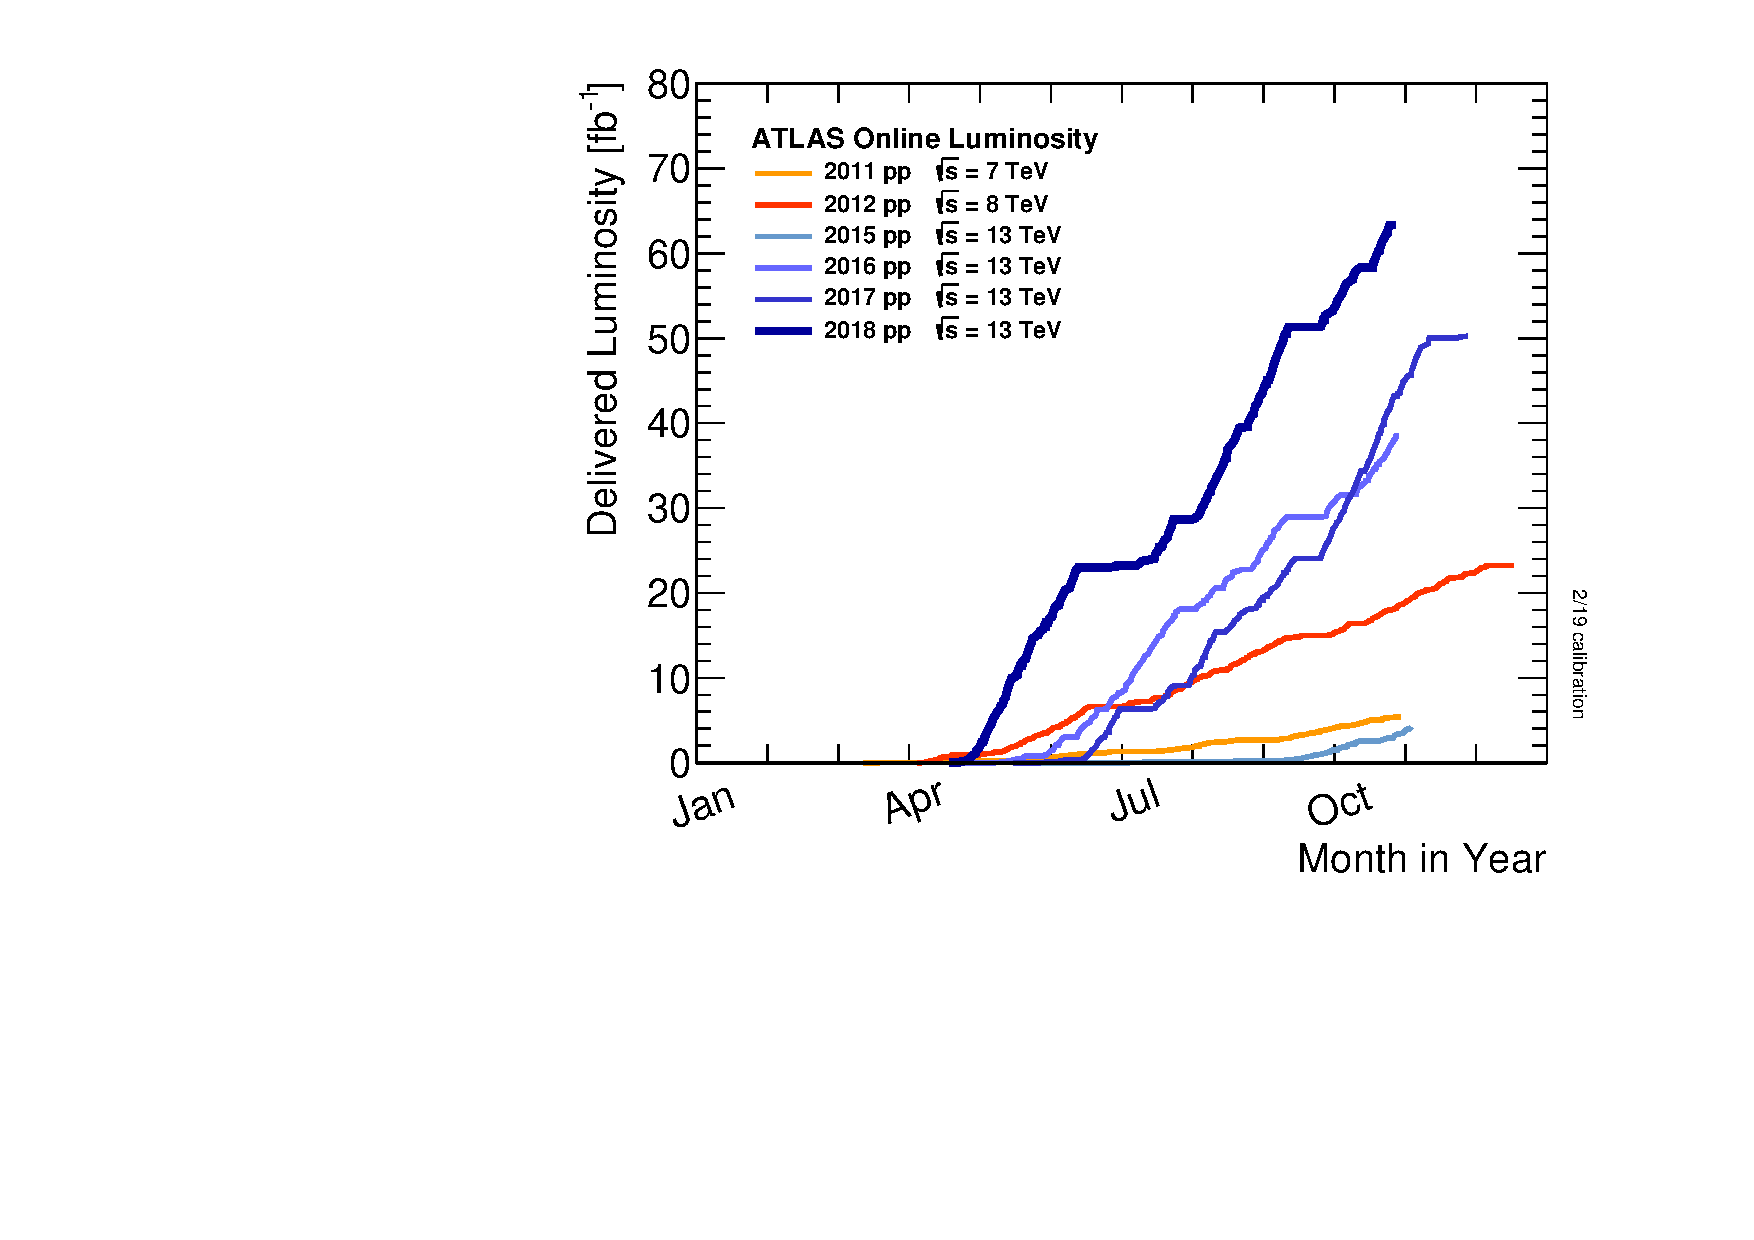
\includegraphics[width=0.5\textwidth]{figures/lhc/intlumivsyear.pdf}}\hfill
\subcaptionbox{2018 Peak Instantaneous Luminosity\label{fig:peakLumiByFill}}{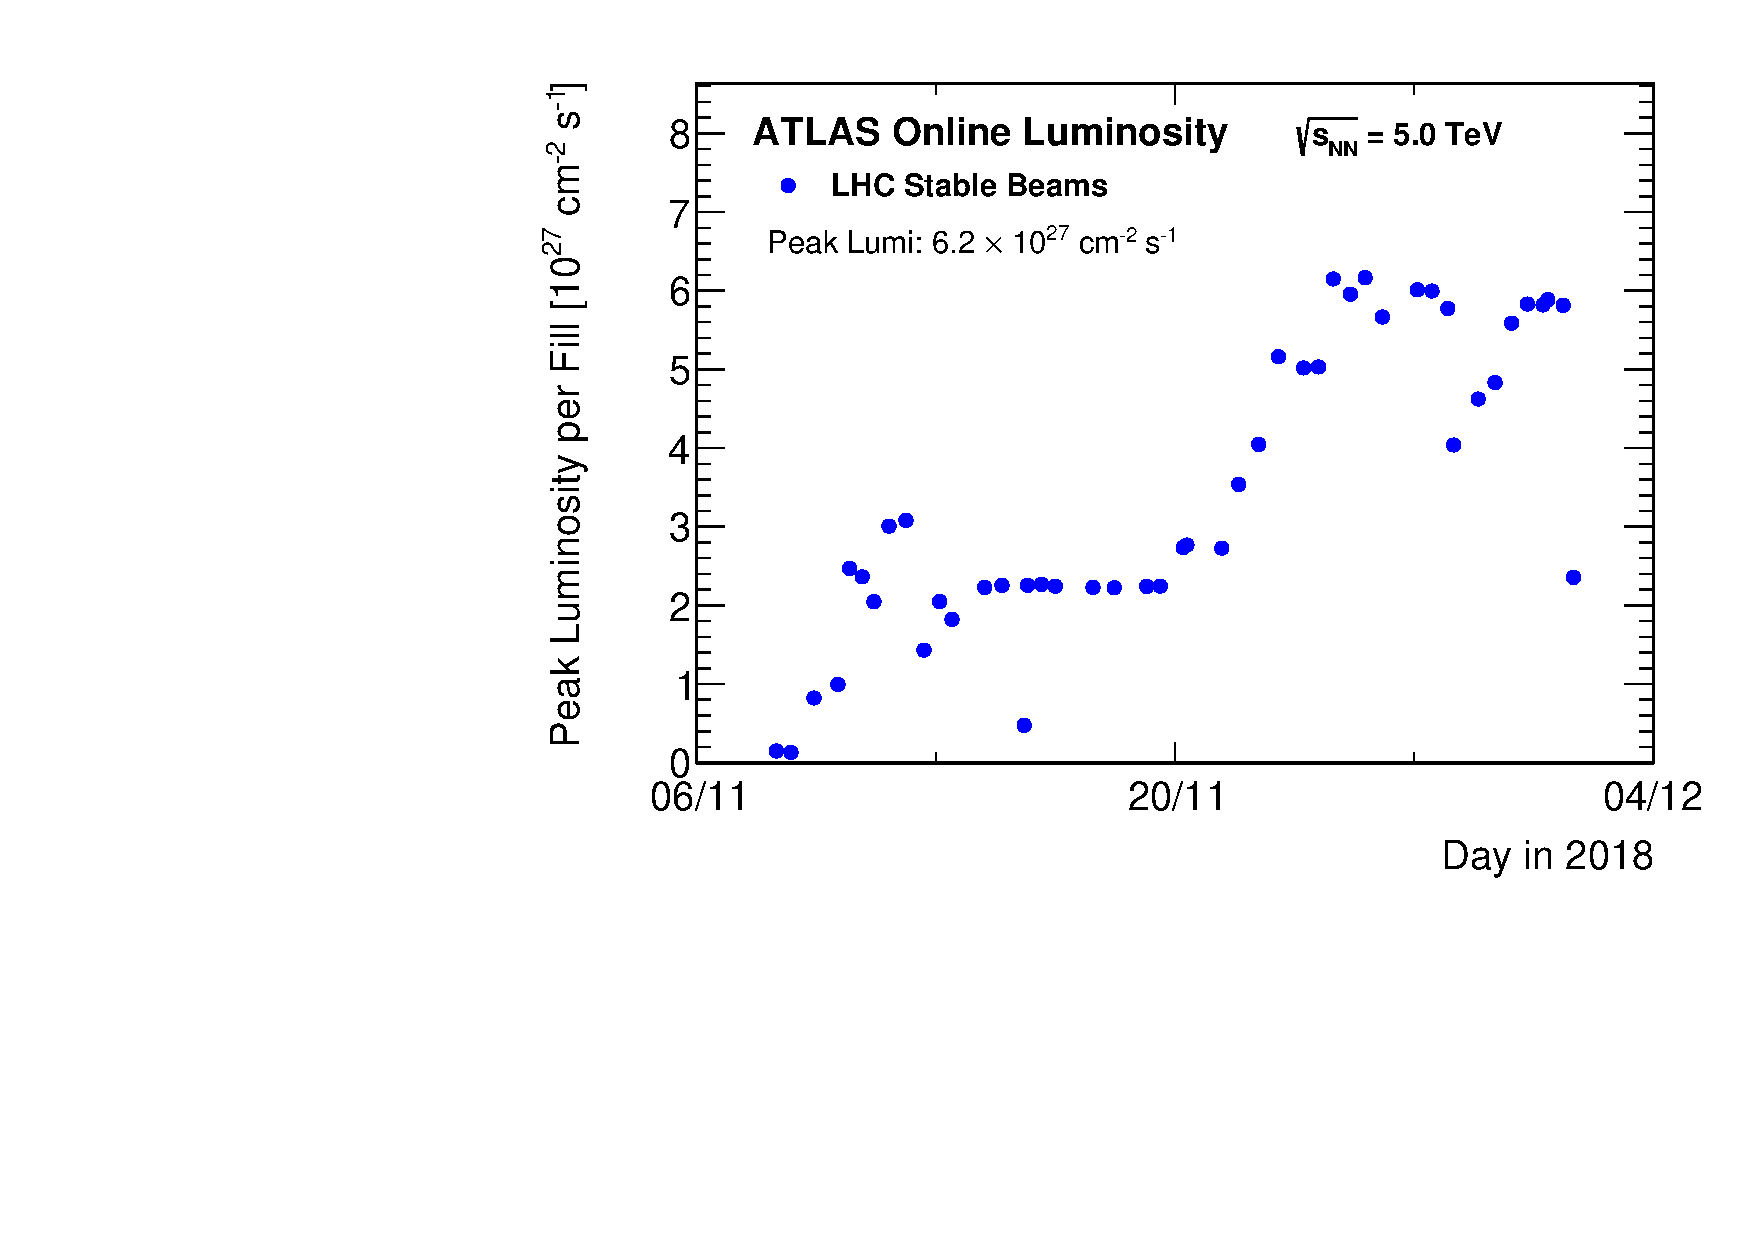
\includegraphics[width=0.5\textwidth]{figures/lhc/peakLumiByFill.pdf}}\hfill
\caption{Luminosity is monitored as both a running total known as the Integrated
Luminosity as depicted in (a) and as an instantaneous quanity as shown in (b).}
\label{fig:luminosity} 
\end{figure}

